\begin{center}
  \Large
  \textbf{BIOGRAFI PENULIS}
\end{center}

\addcontentsline{toc}{chapter}{BIOGRAFI PENULIS}

\vspace{2ex}

\begin{wrapfigure}{L}{0.3\textwidth}
  \centering
  \vspace{-3ex}
  % Ubah file gambar berikut dengan file foto dari mahasiswa
  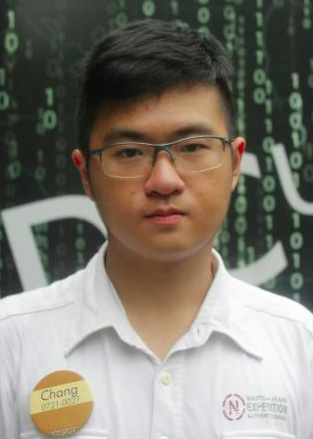
\includegraphics[width=0.3\textwidth]{gambar/chang.png}
  \vspace{-4ex}
\end{wrapfigure}

% Ubah kalimat berikut dengan biografi dari mahasiswa
\hspace{-6ex}Charles Chang atau yang lebih akrab disapa Chang, lahir di Surabaya, Jawa Timur pada 18 Agustus 1999. Merupakan anak pertama dari dua bersaudara. Penulis lulus dari SMP Kristen Petra 5 dan kemudian melanjutkan ke SMA Kristen Petra 1 Surabaya. Penulis merupakan salah satu mahasiswa dari Departemen Teknik Komputer Surabaya, Fakultas Teknologi Elektro dan Informatika Cerdas, Institut Teknologi Sepuluh Nopember. Dalam masa kuliah, penulis sangat tertarik dengan \textit{Machine Learning}, \textit{Image Processing}, dan \textit{Data Science}. Selain itu penulis juga hobi membuat permainan, dan aktif mengikuti lomba membuat permainan di masa kuliah. Bahkan pernah menjadi pemenang juara 3 di MAGE ITS, dan menjadi semi-finalis di Gemastik XII 2019.